\documentclass[a4paper,10pt]{scrartcl}

% Inclusión de paquetes
\usepackage[utf8]{inputenc}
\usepackage[spanish]{babel}

\usepackage{amsmath}
\usepackage{amssymb}
\usepackage{enumerate}
\usepackage{verbatim}
\usepackage{amsthm}
% Imágenes
\usepackage{graphicx}
\usepackage{float}
\usepackage{tikz}
\usetikzlibrary{arrows}

% Enlaces dentro del documento
\usepackage{hyperref}

% Definiciones
\theoremstyle{definition}
\newtheorem*{mydef}{Definición}
%\newtheorem{mydefn}{Definición}
\newtheorem*{theorem*}{Teorema}
\newtheorem{theorem}{Teorema}
\newtheorem*{fact*}{Proposición}
\newtheorem{fact}{Proposición}
\newtheorem*{corollary*}{Corolario}
\newtheorem{corollary}{Corolario}
\newtheorem*{rmk*}{Nota}
\newtheorem*{eg}{Ejemplo}

% Displaystyle por defecto
\everymath{\displaystyle}

% Comandos
\newcommand{\Referencia}[4]{\indent #1, \textbf{#2}. \textit{#3}, \textit{#4}.\\}
\renewcommand\refname{Referencias}
\renewcommand\contentsname{Contenidos}
\documentclass[a4paper,10pt]{scrartcl}

% Inclusión de paquetes
\usepackage[utf8]{inputenc}
\usepackage[spanish]{babel}

\usepackage{amsmath}
\usepackage{amssymb}
\usepackage{enumerate}
\usepackage{verbatim}
\usepackage{amsthm}
% Imágenes
\usepackage{graphicx}
\usepackage{float}
\usepackage{tikz}
\usetikzlibrary{arrows}

% Enlaces dentro del documento
\usepackage{hyperref}

% Definiciones
\theoremstyle{definition}
\newtheorem*{mydef}{Definición}
%\newtheorem{mydefn}{Definición}
\newtheorem*{theorem*}{Teorema}
\newtheorem{theorem}{Teorema}
\newtheorem*{fact*}{Proposición}
\newtheorem{fact}{Proposición}
\newtheorem*{corollary*}{Corolario}
\newtheorem{corollary}{Corolario}
\newtheorem*{rmk*}{Nota}
\newtheorem*{eg}{Ejemplo}

% Displaystyle por defecto
\everymath{\displaystyle}

% Comandos
\newcommand{\Referencia}[4]{\indent #1, \textbf{#2}. \textit{#3}, \textit{#4}.\\}
\renewcommand\refname{Referencias}
\renewcommand\contentsname{Contenidos}
\numberwithin{equation}{section}
\setlength{\parindent}{0cm} % Sin sangrías
\setlength{\parskip}{0.3cm}


\title{Teoría de Colas}
\author{
	Marta Andrés\and
	Ignacio Cordón\and
	Bartolomé Ortiz\and
}
\date{}

\begin{document}
	\maketitle
	
	\begin{center}
		
\includegraphics[width=0.4\textwidth]{./imgs/by-nc-sa.png}
	\end{center}
	
	\tableofcontents
	\pagebreak
	
	\section{Introducción}
	
	\subsection{Distribución exponencial}
	
	Una variable aleatoria continua $X$ tiene distribución exponencial de parámetro $\lambda \ge 0$ si su función de distribución
	$F$ viene dada por:
	
	\[F(x) = \left\{\begin{array}{ll}
	1- e^{-\lambda x} ,& x\ge 0\\
	0 ,& x\le 0
	\end{array}\right.\]
	
	Lo notamos $X \sim exp(\lambda)$
	
	\subsubsection{Propiedad de Markov de la distribución exponencial}
	
	\begin{mydef}
		Decimos que una variable aleatoria $X \ge 0$ tiene la propiedad de Markov si se verifica:
		\[P[X \ge t+h \mid X \ge t] = P[X \ge h] \qquad \forall t,h \in \mathbb{R}_0^{+}\]
	\end{mydef}
	
	Equivalentemente:
	
	\[P[X < t+h \mid X \ge t] = P[X < h] = P[ 0 \le X < h] \qquad \forall t,h \in \mathbb{R}_0^{+}\]
	
	En teoría de colas la propiedad de Markov nos dirá que si el tiempo entre llegadas está distribuido de forma exponencial, 
	la siguiente ocurrencia de un evento es independiente del tiempo de llegada del último evento.
	
	
	\begin{fact}
		Sea $X$ variable aleatoria tal que: $X \sim exp(\lambda)$. Entonces $X$ tiene la propiedad de Markov.
		
		\label{fact:exp-markov}
	\end{fact}
	
	\begin{proof}
		Dados $t,h \in \mathbb{R}$ con $h\ge 0$:
		
		\begin{align*}
		P[X \ge t+h \mid X\ge t]   & = \frac{P[X\ge t+h, X\ge t]}{P[X\ge t]} =  \frac{P[X\ge t+h]}{P[X\ge t]} =\\ 
		& = \frac{e^{-\lambda (t+h)}}{e^{-\lambda t}} = e^{-\lambda h} = P[X\ge h] 
		\end{align*}
	\end{proof}
	
	
	\begin{theorem*}
		Sea $X\ge 0$ variable aleatoria continua con la propiedad de Markov. Entonces $X$ sigue una distribución exponencial.
	\end{theorem*}
	
	\begin{proof}
		Sea la variable aleatoria continua $X\ge 0 $ con función de distribución: \[F(t) = P[X\le t]\]
		
		Se tiene que cumplir por la propiedad de Markov ($t, h\ge 0$):
		
		\[P[X \ge t + h \mid X \ge t] = P[X \ge h]  \Leftrightarrow P[X \ge t + h, X > t] = P[X \ge t] P[X \ge h]\]
		
		Es decir, llamando $G(x) = P[X \ge x] = 1- F(x)$ hemos probado $G(t+h) = G(t) G(h)$ para todo $t, h \ge 0$
		
		Además se tiene claramente que $G$ es decreciente y no negativa.
		
		\[G(0 + 0) = G(0)G(0) \implies G(0) \in \{0,1\}\]
		
		Pero si $G(0) = 0$ entonces $G(t) = G(t+0) = G(t)G(0)$ para todo $t\ge 0$, contradicción por tenerse $G = 1-F$ y $F$ una función de distribución.
		
		Luego $G(0) = 1$
		
		Por inducción se puede probar fácilmente:
		
		\[G(nt) = G((n-1)t) G(t) = \ldots = G(t)^{n}, \qquad \forall t\in \mathbb{R}, n\in \mathbb{N}\]
		
		En particular, $G(n) = G(1)^n$ para cualquier $n\in \mathbb{N}$.
		
		Por último dados $p,q \in \mathbb{N}$:
		
		\[G\left(\frac{p}{q}\right)^q = G\left(\frac{p}{q} q\right) = G(1)^p \implies G\left(\frac{p}{q}\right) = G(1)^{\frac{p}{q}}\]
		
		Luego como $F$ es continua, $G$ lo es, y para cada $x \in \mathbb{R}$ podemos tomar $\{r_n\} \rightarrow x$ sucesión de racionales,
		y se tiene:
		
		\[G(x) = G(1)^x = e^{\log(G(1)) x}\]
		
		Es decir:
		
		\[F(x) = 1 - G(x) = 1 - e^{\log(G(1)) x}\]
		
		donde $-\lambda = \log(G(1)) \le \log(G(0)) = 0$ por el decrecimiento de $G$
		
	\end{proof}
	
	
	\subsection{Procesos de Poisson}
	
	\subsubsection{Notación O pequeña}
	\begin{mydef} 
		Una función $f$ se dice $o(h)$ (formalmente $f\in o(h)$) y lo notamos $f=o(h)$ si se verifica:
		
		\[\lim_{h\rightarrow 0} \frac{f(h)}{h} = 0\]
	\end{mydef}
	
	Es decir, una función $f(h)$ es $o(h)$ si al compararla con un $h$ suficientemente pequeño, podemos despreciar su
	valor.
	
	\begin{fact*}
		Dados $c_1, \ldots c_n \in \mathbb{R}$, $f_1, \ldots f_n \in o(h)$, entonces $\sum_{i=1}^{n} c_i f_i = o(h)$
	\end{fact*}
	
	\begin{proof}
		\[\lim_{h\rightarrow 0} \frac{\sum_{i=1}^{n} c_i f_i}{h} = \sum_{i=1}^{n}{c_i \lim_{h\rightarrow 0} \frac{f_i}{h}} = 0\]
	\end{proof}
	
	\subsubsection{Proceso de Poisson}
	
	\begin{mydef} \textbf{Proceso de conteo}\\
		Sea $\{N_t\}_{t\ge 0}$ proceso estocástico discreto. Se dice que es proceso de conteo si se verifica:
		\begin{enumerate}
			\item No negatividad: $N_t \in \mathbb{N}\cup\{0\}, \quad \forall t\ge 0$. Además: $N_0=0$
			\item Monotonía: $N_s \le N_t, \quad \forall s \le t$
		\end{enumerate}
		
		$N_t$ indica el número de eventos que han ocurrido en el intervalo $[0,t]$. Por tanto $N_t- N_s$, con $t\ge s$
		indica el número de eventos que han ocurrido en $]s,t]$.
	\end{mydef}
	
	
	\begin{mydef} \textbf{Proceso de Poisson}\\
		Un proceso de conteo $\{N_t\}_{t\ge 0}$ se dice que es de Poisson de parámetro $\lambda > 0$ si se verifica:
		
		\begin{enumerate}
			\item El proceso tiene incrementos independientes: dados $0 \le t_1 < \ldots < t_n$, se verifica que
			las variables $N_{t_1}, N_{t_2} - N_{t_1}, \ldots, N_{t_n}- N_{t_{n-1}}$ son independientes. Esto es, el número de eventos
			que se producen en intervalos disjuntos es independiente.
			\item El proceso tiene incrementos estacionarios: $dist(N_{t+h} - N_t)$ es la misma para cualesquiera
			$t\ge 0, h\ge 0$.
			\item $P[N_h = 1] = \lambda h + o(h)$, es decir, la probabilidad de que ocurra un evento en un intervalo de
			tiempo de longitud $h$ es casi proporcional a $h$, salvo por un término despreciable en comparación con dicho $h$, para
			$h$ suficientemente pequeño.
			\item $P[N_h \ge 2] = o(h)$.
		\end{enumerate}
		
		Se deduce que: 
		\[P[N_h = 0] = 1 - P[N_h=1] - P[N_h \ge 2] = 1 -\lambda h - o(h)\]
	\end{mydef}
	
	
	La mayoría de modelos de colas asumen una distribución exponencial para tiempos entre llegadas y tiempos 
	de servicio, o equivalentemente una distribución de Poisson para frecuencias de llegada y servicio.
	
	\begin{theorem}
		Sea $\{N_t\}_{t\ge 0}$ un proceso de Poisson de parámetro $\lambda > 0$. Entonces la variable aleatoria $Y_t = N_t - N_0 = N_t$ que
		describe el número de eventos en cualquier intervalo de longitud $t > 0$ tiene una distribución de Poisson de parámetro
		$\lambda t$:
		
		\[P[Y_t = k] = P[N_t = k] = e^{-\lambda t} \frac{(\lambda t)^k}{k!}, \quad k\ge 0\]
		
		\label{th:poisson-probs}
	\end{theorem}
	
	
	\begin{theorem*}
		Sea $\{N_t\}_{t\ge 0}$ proceso de conteo. Sea $\{t_n\}_{n\ge 1}$ sucesión real estrictamente creciente y positiva, 
		que representa los tiempos de eventos, es decir \[t_n = \min \{t \ge 0: N_t = n\}\]
		
		LLamando $\tau_1= t_1, \tau_{n+1} = t_{n+1} - t_{n}, \quad \forall n\in \mathbb{N}$ tiempos entre llegadas. Entonces equivalen:
		
		\begin{itemize}
			\item $\{N_t\}_{t\ge 0}$ es proceso de Poisson.
			\item Los tiempos entre llegadas $\{\tau_n\}$ son variables exponenciales i.i.d. de media $\frac{1}{\lambda}$, esto es,
			$\tau_n \sim exp(\lambda)$.
		\end{itemize}
		
	\end{theorem*}
	
	%% Prueba: falta por hacer.
	
	\begin{theorem*}
		Sea $\{N_t\}_{t\ge 0}$ proceso de Poisson donde un evento ha tenido lugar en $[0,t]$. Entonces siendo $Y$ la variable
		describiendo el tiempo de ocurrencia de dicho evento en el intervalo $[0,t]$, se tiene $Y \sim U([0,t])$.
	\end{theorem*}
	
	%% Prueba: falta por hacer.
	
	\subsection{Procesos de nacimiento y muerte}
	
	El parámetro $\lambda$ de un proceso de Poisson $\{N_t\}_{t\ge 0}$ puede ser visto como una tasa de nacimiento, ya que la probabilidad
	de que ocurra un evento en un intervalo de longitud $h > 0$ es $P[N_h-N_0=1] = \lambda h e^{-\lambda h} = \lambda h + o(h)$.
	Cuando suponemos que el parámetro no es constante, sino que depende de $n$ (cantidad de eventos que se han producido hasta el momento), esto
	es $\lambda_n$, entonces la cantidad de nacimientos (eventos producidos) en un intervalo de longitud $h$ es $\lambda_n h + o(h)$. Si además
	establecemos que se pueden producir muertes con una tasa $\mu_n$, donde la probabilidad de que se produzca una muerte en un intervalo de longitud
	$h$ es $\mu_n h + o(h)$ tenemos un proceso de nacimiento y muerte.
	
	\begin{mydef}
		Sea una cadena de Markov $\{N_t\}_{t\ge 0}$ con espacio de estados $\mathbb{N}\cup \{0\}$, donde el espacio de estados representa el número de individuos
		de un sistema (población). Entonces $\{N_t\}_{t\ge 0}$ se dice proceso de nacimiento y muerte si existen tasas no negativas de nacimiento y muerte,
		$\{\lambda_n\}_{\mathbb{N}\cup \{0\}}$ y $\{\mu_n\}_{\mathbb{N}\cup \{0\}}$ y se verifica:
		
		\begin{enumerate}
			\item La población puede aumentar o decrecer únicamente de uno en uno.
			\item Si el sistema está en estado $n\ge 0$ entonces el tiempo hasta que el sistema está en estado $n+1 \ge 0$ es una variable aleatoria exponencial
			de paŕámetro $\lambda_n$.
			\item Si el sistema está en estado $n\ge 1$ entonces el tiempo hasta que el sistema está en estado $n-1 \ge 0$ es una variable aleatoria exponencial
			de paŕámetro $\mu_n$.
			\item Cualesquiera dos transiciones son independientes.
		\end{enumerate}
	\end{mydef}
	
	Llamando $P_n(t) = P[N_t = n]$ se verifica:
	
	Sea $h>0$ suficientemte pequeño. Entonces la probalidad $P_n(t+h)$ viene dada por la suma de la probabilidad de 
	los siguientes hechos disjuntos:
	
	\begin{enumerate}
		\item En $t$ el sistema tenía población $n$ y no se han producido muertes ni nacimientos hasta $t+h$, esto es:
		\begin{align*}
		&  P[N_{t+h}=n] \cdot (1-\lambda_n h + o(h)) \cdot (1-\mu_n h + o(h))= \\
		&= P_n(t)[1+\mu_n h + o(h) -\lambda_n h + \lambda_n \mu_n h^2 + o(h)] = \\
		&= P_n(t)(1-\lambda_n h - \mu_n h) + o(h)
		\end{align*}
		
		Donde se ha usado independencia de nacimientos y muertes y agrupación de todas las funciones que son $o(h)$
		
		\item En $t$ el sistema tenía población $n-1$ y se ha producido un único nacimiento entre $t$ y $t+h$:
		
		\[P_{n-1}(t) (\lambda_{n-1}h + o(h)) = P_{n-1}(t) \lambda_{n-1} h + o(h)\]
		
		\item En $t$ el sistema tenía población $n+1$ y se ha producido una única muerte entre $t$ y $t+h$:
		
		\[P_{n+1}(t) (\mu_{n+1} h + o(h))\]
		
		\item La probabilidad de que ocurran 2 o más transiciones entre $t$ y $t+h$ es $o(h)$ por hipótesis.
	\end{enumerate}
	
	
	Sumando y agrupando funciones $o(h)$:
	
	\[P_n(t+h) = [1-\lambda_n h -\mu_n h] P_n(t) + \lambda_{n-1} h P_{n-1}(t) + \mu_{n+1} h P_{n+1}(t) + o(h)\]
	
	
	Que diviendo por $h$ en ambos términos y operando, da lugar a:
	
	\[\frac{P_n(t+h) - P_n(t)}{h} = -(\lambda_n + \mu_n) P_n(t) + \lambda_{n-1} P_{n-1}(t) + \mu_{n+1}P_{n+1}(t) + \frac{o(h)}{h}\]
	
	Tomando límite en $h\rightarrow 0$ llegamos a:
	
	\begin{equation}
	\frac{\partial P_n(t)}{\partial t} = -(\lambda_n + \mu_n) P_n(t) + \lambda_{n-1}P_{n-1}(t) + \mu_{n+1}P_{n+1}(t)
	\label{eq:recpn(t)}
	\end{equation}
	
	En el caso particuar $n=0$, tenemos $\mu_o = 0$ y $P_{-1}(t) = 0$. Por tanto:
	
	\begin{equation}
	\frac{\partial P_0(t)}{\partial t} = -\lambda_0 P_0(t) \mu_{1}P_{1}(t)
	\label{eq:recp0(t)}
	\end{equation}
	
	
	Supongamos en lo que sigue que existe la distribución límite (entonces existiría la estacionaria), esto es 
	$\lim_{t\rightarrow \infty}\{P_n(t)\} = p_n$ y haciendo $t\rightarrow \infty$ en \eqref{eq:recpn(t)},
	y en \eqref{eq:recp0(t)} llegamos a que:
	
	\begin{align*}
	0 &= \lambda_{n-1} p_{n-1} + \mu_{n+1} p_{n+1} - (\lambda_n + \mu_n) p_n, \quad n\ge 1\\
	0 &= \mu_1 p_1 -\lambda_0 p_0, \quad n=0
	\end{align*}
	
	Justificamos que la parte izquierda se hace cero: habríamos llegado a que $\frac{\partial P_n(t)}{\partial t}$ tiende a una constante $C$,
	pero la $P_n$ tiende a $p_n$, luego no es difícil demostrar que $C$ debe ser 0.
	
	Veamos por inducción que: $p_n = p_0 \prod_{i=1}^n \frac{\lambda_{i-1}}{\mu_i}, \quad n\ge 1 \label{p_n=p_0*}$.
	
	\begin{proof}
		Los casos $n=0, n=1$ cumplen trivialmente la recurrencia. Para $n>0$, aplicando hipótesis de inducción a $p_{n-1}, p_{n}$:
		
		\begin{align*}
		p_{n+1} &= \frac{\lambda_n + \mu_n}{\mu_{n+1}} p_n - \frac{\lambda_{n-1}}{\mu_{n+1}}p_{n-1} = \\
		&= \frac{\lambda_n + \mu_n}{\mu_{n+1}} p_0 \prod_{i=1}^n \frac{\lambda_{i-1}}{\mu_i} - 
		\frac{\lambda_{n-1}}{\mu_{n+1}} p_0 \prod_{i=1}^{n-1} \frac{\lambda_{i-1}}{\mu_i} = \\
		&= \frac{\lambda_n}{\mu_{n+1}} p_0 \prod_{i=1}^n \frac{\lambda_{i-1}}{\mu_i} + 
		\frac{\mu_n \lambda_{n-1}}{\mu_{n+1}\mu_n} p_0 \prod_{i=1}^{n-1} \frac{\lambda_{i-1}}{\mu_i} - 
		\frac{\lambda_{n-1}}{\mu_{n+1}} p_0 \prod_{i=1}^{n-1} \frac{\lambda_{i-1}}{\mu_i} = \\
		&= \frac{\lambda_n}{\mu_{n+1}} p_0 \prod_{i=1}^n \frac{\lambda_{i-1}}{\mu_i} = p_0 \prod_{i=1}^{n+1} \frac{\lambda_{i-1}}{\mu_i}
		\end{align*}
	\end{proof}
	
	Además, las probabilidades deben sumar $1$, esto es:
	
	\begin{equation}
	1 = \sum_{n=0}^{\infty} p_n = p_0 \underbrace{\left(1 + \sum_{n=1}^{\infty} \prod_{i=1}^n \frac{\lambda_{i-1}}{\mu_i} \right)}_{Z}
	\label{eq:stabseries}
	\end{equation}
	
	Que la serie $Z$ sea convergente es condición necesaria para que exista la distribución límite. 
	De hecho, también es condición suficiente (se puede probar por teorema de ergodicidad, aunque su prueba queda
	fuera del nivel de estos apuntes). Si dicha distribución existe se tendría: 
	
	\begin{equation}
	p_0 = Z^{-1} 
	\label{eq:relp0}
	\end{equation}
	
	Intuitivamente, cuando la serie $Z$ converge, tenemos que la probabilidad límite de que el 
	sistema esté vacío y no haya clientes esperando en la cola es positiva, y por tanto el sistema 
        es estable. Cuando esta serie diverge, es un indicativo de que el modelo de colas
	es inestable.
	
	
	\section{El modelo de un proceso de colas}
	\subsection{Definición}
	Un modelo de colas es un sistema que modela clientes (que también pueden ser vistos como peticiones o eventos) que llegan a una cola,
	donde existe un tiempo de espera en cola, y un tiempo de servicio. Su funcionamiento básico se 
	ilustra en la figura \ref{fig:encolado}. Debemos considerar una serie de variables aleatorias que permitan
	explicar y estudiar el comportamiento de la cola. Las variables límites se definen, claro está, cuando esta 
	tenga sentido:
	
	\begin{itemize}
		\item [$c$]
		Número (fijo) de servidores o canales en el sistema, $c\in \mathbb{N} \cup \{+\infty\}$
		\item [$\tau$]
		Variable aleatoria que describe el tiempo entre llegadas (de clientes).
		\item [$S$]
		Variable aleatoria que describe el tiempo de servicio.
		\item [$Q$]
		Variable aleatoria que describe el tiempo que espera un cliente en la cola.
		\item [$N_{S,t}$]
		Variable aleatoria que describe el número de clientes que están siendo servidos en el instante $t$.
		\item [$N_{Q,t}$]
		Variable aleatoria que describe el número de clientes en la cola (esperando a ser servidos) en el instante $t$.
	\end{itemize}
	
	\begin{figure}[h]
		\centering
		\begin{tikzpicture}
		\draw (20,5.5) rectangle (22,6);
		\node [above] at (21,5.5) {Servidor 1};
		\draw (20,4.5) rectangle (22,5);
		\node [above] at (21,4.5) {Servidor 2};
		\draw [dotted, ultra thick] (21,4.15) -- (21,3.85);
		\draw (20,3) rectangle (22,3.5);
		\node [above, black] at (21,3) {Servidor $c$};
		
		\draw [fill] (19.5,5.75) circle [radius=0.1];
		\draw [fill=white] (19.5,4.75) circle [radius=0.1];
		\draw [fill] (19.5,3.25) circle [radius=0.1];
		\draw [dashed, black] (19.25,3) rectangle (19.75,6);
		\node [below, black] at (19.5,3) {$N_{S,t}$};
		
		\draw [latex-latex, black] (19.25,6.5) -- (22,6.5);
		\draw [black] (19.25,6) --(19.25,6.6);
		\draw [black] (22,6) --(22,6.6);
		\node [above, black] at (20.7,6.5) {$S$};
		
		\draw (22.15,6) -- (22.5,6) -- (22.5,3) -- (22.15,3);
		\draw [-latex] (22.5,4.5) -- (23.5,4.5);
		
		\draw (19,6) -- (18.65,6) -- (18.65,3) -- (19,3);
		\draw [-latex] (18,4.5) -- (18.65,4.5);
		\draw [fill] (18,4.5) circle [radius=0.1];
		\draw [fill] (17.6,4.5) circle [radius=0.1];
		\draw [dotted, ultra thick] (17,4.5) -- (17.3,4.5);
		\draw [fill] (16.7,4.5) circle [radius=0.1];
		\draw (16,4.5) -- (16.6,4.5);
		\draw [black] (16.6,4.3) -- (16.6,4.1) -- (18.1,4.1) -- (18.1,4.3);
		\node [below, black] at (17.35,4.1) {$N_{Q,t}$};
		
		\draw [latex-latex, black] (16.05,5) -- (18.6,5);
		\node [above, black] at (17.34,5) {$Q$};
		
		\draw (16,2) rectangle (23,7.5);
		\node [above] at (19.5,7.5) {Modelo de cola};
		
		\draw (12,4.25) rectangle (13.6,4.75);
		\node [above] at (12.8,4.25) {Fuente};
		\draw [-latex] (13.6,4.5) -- (16,4.5);
		\draw [fill] (14.25,4.5) circle [radius=0.1];
		\draw [fill] (15.25,4.5) circle [radius=0.1];
		
		\draw [latex-latex, black] (14.25,5) -- (15.25,5);
		\draw [black] (14.25,4.65) --(14.25,5.1);
		\draw [black] (15.25,4.65) --(15.25,5.1);
		\node [above, black] at (14.75,5) {$\tau$};
		\end{tikzpicture}
		\caption{El modelo de un proceso de colas.}
		\label{fig:encolado}
	\end{figure}
	
	De ellas se derivan las siguientes variables, también relevantes:
	\begin{itemize}
		\item [$\lambda$]
		Frecuencia o tasa media de llegadas de clientes al sistema: $\lambda = 1/E[\tau]$.
		\item [$\mu$]
		Frecuencia o tasa media de servicio de los servidores del sistema: $\mu = 1/E[S]$.
		\item [$\rho$]
		Aprovechamiento de los servidores, esto es, la proporción de tiempo que los servidores están trabajando: $\rho = \frac{\lambda}{c\mu}$.
		\item [$W_S$]
		Tiempo medio que está siendo servido un cliente: $W_S  = E[S]$.
		\item [$W_Q$]
		Tiempo medio que está un cliente en la cola: $W_Q = E[Q]$.
		\item [$W$]
		Tiempo de espera. Variable aleatoria que describe el tiempo total que un cliente está en el sistema: $W = Q+S$.
		\item [$W_W$]
		Tiempo medio (de espera) que está un cliente en el sistema: $W_W = E[W]$.
		\item [$N_S$]
		Variable aleatoria que describe el número de clientes siendo servidos con el sistema en equilibrio: $N_S = \lim_{t \rightarrow \infty} N_{s,t}$.
		\item [$L_S$]
		Número medio de clientes siendo servidos con el sistema en equilibrio: \\ $L_S = E[N_S]$.
		\item [$N_Q$]
		Variable aleatoria que describe el número de clientes en la cola con el sistema en equilibrio: $N_Q = \lim_{t \rightarrow \infty} N_{Q,t}$.
		\item [$L_Q$]
		Número medio de clientes en la cola con el sistema en equilibro: $L_Q = E[N_Q]$.
		\item [$N_t$]
		Variable aleatoria que describe el número de clientes en el sistema en el instante $t$: $N_t = N_{Q,t} + N_{S,t}$.
		\item [$N$]
		Variable aleatoria que describe el número de clientes en el sistema con el sistema en equilibrio $N = N_Q + N_S$.
		\item [$L$]
		Número medio de clientes en el sistema en equilibrio: $L = E[N]$.
		\item [$P_n(t)$]
		Probabilidad de que haya $n$ clientes en el sistema en el instante $t$: es la función masa de probabilidad de $N_t$.
		\item [$p_n$]
		Probabilidad de que haya $n$ clientes en el sistema con el sistema en equilibrio: $p_n = \lim_{t \rightarrow \infty} P_n(t)$ es la función masa de probabilidad de $N$.
	\end{itemize}
	
	\subsection{Características}
	\subsubsection{Modelo de llegadas}
	La capacidad de un sistema de colas para poder proporcionar servicio a los clientes no depende solo de la tasa media
	de llegadas de un sistema de colas, sino también del modo en que las peticiones llegan. De esta forma, podemos
	tener que las peticiones llegan de uno en uno, o en paquetes de peticiones.
	
	Dados $0=t_0 < t_1 < t_2 < t_n < \ldots$, y $\tau_n = t_n - t_{n-1}, \tau_0$ tiempos entre llegadas, asumimos por hipótesis
	que las $\tau_n$ son variables aleatorias i.i.d. Nótese que tanto los $\{t_n\}$ como los $\{\tau_n\}$ son
	variables aleatorias.
	
	\begin{mydef}
		LLamamos modelo de llegadas a la distribución $A(t)$ de los tiempos entre llegadas $\{\tau_n\}$.
	\end{mydef}
	
	La distribución de los tiempos de llegada $\{t_n\}$ está determinada por la distribución de los tiempos entre
	llegadas $\{\tau_n\}$. 
	
	\begin{mydef}
		El modelo de llegadas se dice:
		
		\begin{enumerate}
			\item Estacionario, cuando no depende del tiempo (por ejemplo cuando existe una distribución límite y hablamos
			del modelo de llegadas de dicha distribución límite).
			\item Transitorio, en caso opuesto.
		\end{enumerate}
	\end{mydef}
	
	
	\begin{mydef}
		Para un modelo de llegadas, sea $A(t)$ función de distribución de los $\tau_n$. 
		El modelo de llegadas se dice:
		
		\begin{enumerate}
			\item Aleatorio o de Poisson: si $A(t) = 1 - e^{-\lambda t}$.
			\item Determinístico: si $A(t) = \left\{\begin{array}{ll}
			0 & t<s \\
			1 & t\ge s
			\end{array}\right.$ con $s$ fijo.
			
		\end{enumerate}
	\end{mydef}
	
	
	\subsubsection{Modelo de servicio}
	
	Se pueden efectuar unas definiciones análogas para modelo determinístico, aleatorio y régimen estacionario y transitorio
	de servicio a las que se han hecho con el modelo de llegadas.
	
	\begin{eg} \textbf{Caso particular, modelo de Poisson de servicio}
		
		Supongamos que el modelo de colas tiene $k$ servidores o canales para atender peticiones, y el tiempo que 
		tarda cada uno en atender una petición $T_i, i=1,\ldots k$ sigue una distribución exponencial de parámetro $\bar{\mu}$.
		Entonces el tiempo hasta terminar de atender una petición es $T = min\{T_1, \ldots T_n\}$. Por propiedades de la
		distribución exponencial deducimos que $T$ sigue una distribución exponencial de parámetro $\mu = n \bar{\mu}$
		
		La función de distribución de $W_S$ por tanto sería $W_S[t] = P[S\le t] = 1 - e^{-\mu t}$.
		
	\end{eg}
	
	\subsubsection{Capacidad del sistema}
	
	Sea $S\subseteq \mathbb{N}$ el menor espacio de estados sobre el que está definido el proceso estocástico $\{N_{Q,t}\}_{t\ge 0}$ . 
	Se llama capacidad al tamaño máximo de la cola de peticiones, esto es $M = \max S \in \mathbb{N} \cup \{+\infty\}$. 
	Por tanto no puede tenerse que en ningún tiempo $N_{Q,t}$ tome un valor mayor que $M$, y si llegara una
	petición cuando la cola tiene tamaño $M$, se rechazaría dicha petición.
	
	\subsubsection{Comportamiento de los clientes}
	Podemos considerar que los clientes que llegan a la cola pueden efectuar:
	
	\begin{itemize}
		\item Oposición: una petición se retira en la llegada (por ejemplo en casos en los que la cola sea muy larga
		y el cliente se abstenga de entrar).
		\item Retirada: la petición entra a la cola, pero tras un tiempo de espera, la deja.
		\item Recolocación: si hay varias colas paralelas, los clientes se pueden cambiar de una cola a otra.
		\item Priorización: algunos clientes pueden tener mayor prioridad que otros al ser servidos.
	\end{itemize}
	
	\subsubsection{Disciplina de la cola}
	Se pueden tener distintas formas de elegir de la cola el siguiente cliente a ser servido. Consideramos las siguientes estrategias:
	\begin{itemize}
		\item FIFO (First in, first out): es la cola tradicional, en la que el cliente que lleva más tiempo esperando en la cola es el siguiente en ser servido.
		\item LIFO (Last in, first out): el cliente que lleva menos tiempo esperando en la cola es el siguiente en ser servido.
		\item SIRO (Service in random order): se escoge un cliente al azar de entre todos los de la cola, con probabilidad uniforme.
		\item PRI (Priority  service): los clientes tienen asignado un nivel de prioridad y se elige el cliente con mayor prioridad de la cola. En caso de haber varios con la misma probabilidad, se usa alguna de las disciplinas anteriores para elegir entre ellos.
	\end{itemize}
	
	\subsection{Notación de Kendall}
	
	Se utiliza para describir las características de una cola de forma breve la notación de Kendall, de la forma $A/B/c/K/m/Z$, donde:
	\begin{itemize}
		\item $A$ y $B$ describen $\tau$ (el tiempo entre llegadas) y $S$ (el tiempo de servicio) respectivamente, siendo los símbolos más comunes:
		\begin{itemize}
			\item [$G$]
			General, sólo se asume que $\tau_n$ o $S_n$ son independientes.
			\item [$D$]
			Determínistica, donde $\tau$ es constante.
			\item [$M$]
			De Markov, esto es, se usa la distribución exponencial para dar un proceso de llegadas llamado de Poisson o aleatorio.
			%% Estas dos no aparecen en en el apartado 2.1.1, ponerlas?
			%% \item [$E_k$] Erlang-k
			%% \item [$H_k$] k-stage hyperexponential
		\end{itemize}
		\item $c$ describe el número de servidores, que puede ir desde 1 hasta infinito (aunque en teoría no se puede tener un número infinito de servidores, en la práctica se puede tener una cantidad de servidores suficientemente grande como para parecer infinita).
		\item $K$ describe la capacidad máxima del sistema, esto es, el número máximo de clientes que puede haber en el sistema entre la cola y el servicio.
		\item $m$ describe el tamaño de la población en la fuente, que puede ir desde 1 hasta infinito.
		\item $Z$ describe la disciplina de la cola, con las siglas usadas anteriormente (u otras equivalentes, mientras no haya ambigüedad).
	\end{itemize}
	
	A menudo, se asume que $K$ y $m$ son infinitos y $Z$ es de tipo FIFO, y se usa una notación acortada de la forma $A/B/c$.
	
	\subsection{Medidas de efectividad}
	Se pueden considerar disintos valores como medidas de efectividad del sistema, entre ellos, los siguientes:
	\begin{itemize}
		\item $\rho$:
		Aprovechamiento de los servidores, esto es, la proporción de tiempo que los servidores están trabajando: 
		$\rho = \frac{\lambda}{c\mu}$. Cuanto más alta mayor es la eficiencia de los servidores, pero 
		si $\rho > 1$ significa que el sistema está sobrecargado y aumentará el número de clientes en la cola, 
		ya que entran clientes al sistema más rápido que salen.
		\item $W_W$:
		Tiempo medio de un cliente en el sistema. Naturalmente, se desea minimizar el tiempo que tarda un 
		cliente en ser servido.
		\item $W_Q$:
		Tiempo medio de un cliente en la cola. Similar al anterior, pero en algunos casos puede interesar más 
		el tiempo de espera en la cola solamente. Por ejemplo, en el caso de la cola en un supermercado, un 
		cliente estará insatisfecho si tiene que esperar mucho tiempo en la cola, pero mientras está siendo 
		servido está ocupado y no lo percibe como tiempo de espera.
		\item $\pi_{W_W} \lbrack 90 \rbrack$:
		Percentil 90 del tiempo total en el sistema $W_W$. En lugar de usar la media que puede ser afectada por 
		casos extremos, se utiliza el tiempo de espera de una gran parte de los clientes, pudiendo variar el 
		percentil que se considera según se desee.
		\item $\pi_{W_Q} \lbrack 90 \rbrack$:
		Percentil 90 del tiempo de espera en la cola $W_Q$. Análogamente al anterior, pero una vez más teniendo en
		cuenta únicamente el tiempo de espera en la cola y no el total.
		\item $L$:
		Número medio de clientes en el sistema. En general, cuantos más clientes haya en el sistema mayor será su
		tiempo de espera. Sin embargo, si hay muchos servidores no necesariamente se puede optimizar el sistema,
		por tanto mientras $L<c$ no necesariamente es ineficiente el sistema.
		\item $L_Q$:
		Número medio de clientes en la cola. Como se explica en el punto anterior, el número medio de clientes en 
		el sistema no necesariamente es representativo, y puede ser más útil considerar el número medio de clientes
		esperando en la cola, excluyendo así los que están siendo servidos.
		\item $p_n$:
		Probabilidad de que haya $n$ clientes en el sistema (en el estado de equilibrio). En general, interesa 
		conocer su función de distribución para que la probabilidad de que haya $n$ o menos clientes en el sistema
		sea lo más alta posible para un $n$ adecuadamente pequeño.
		\item $a$:
		La intensidad de tráfico se define como $a= W_S/E[\tau]$. Se da que es proporcional al aprovechamiento de
		los servidores, $a = \rho c$, luego ambas se pueden usar como medida de eficiencia, dependiendo si se 
		quiere considerar el número de servidores en la medida o no.
	\end{itemize}
	
	\section{Leyes de Little}
	Para $n \geq 1$, llamemos al cliente $n$-ésimo, el cual llega en el instante $t_n$, nombremos $W_n$ al tiempo 
	de espera del cliente con lo cual es inmediato deducir, que nuestro cliente abandonará la cola en el instante
	$t_n + W_n$, donde $0 = t_0 \leq t_1 \leq t_2 \leq... $.
	
	Es inmediato tambien que podemos definir una función indicadora que refleje si el $c_n$ está o no en el
	sistema:
	
	Indicador: $I_n(t) = \left\{\begin{array}{cc}
	1, & t_n \leq t <t_n + W_n\\
	0, & \textrm{en otro caso}
	\end{array}\right.$, de donde  $\int_{0}^{\infty} I_n(t)dt=W_n$.
	
	Sea $\Delta(t) = max \{i: t_n \leq t\}$ el número de llegadas en tiempo $t$. El número de clientes en el sistema
	viene dado por:
	
	\[N_t = \sum_{i=1}^{\Delta(t)} I_n(t)\]
	
	A partir del tiempo de llegada ${t_n}$ y del tiempo de servicio ${W_n}$ del cliente $n$-ésimo, podemos 
	construir ${N_t}$ para todo $t$. Visualmente podemos entender de forma sencilla estos conceptos si trazamos 
	${\Delta (t)}$ como una función escalonada y mostramos un tiempo de espera del cliente.
	
	\begin{figure}[H]
		\begin{center}
			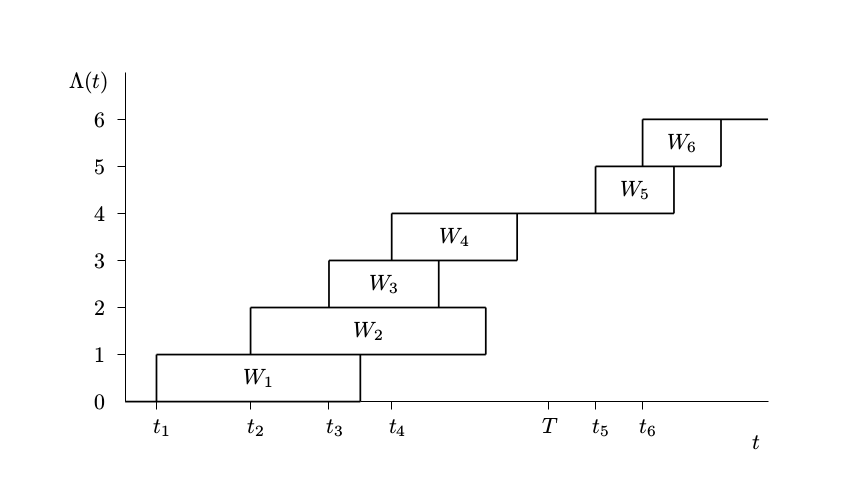
\includegraphics[width=\textwidth]{./imgs/fig1.png}
			\caption{Trayectoria de $\Delta(t)$}
			\label{fig:deltat}
		\end{center}
	\end{figure}
	
	A su vez podemos representar $N_t$ como una función escalonada (cuya información será obviamente menor que la primera figura) 
	representando únicamente el número de personas en el sistema.
	
	\begin{figure}[H]
		\begin{center}
			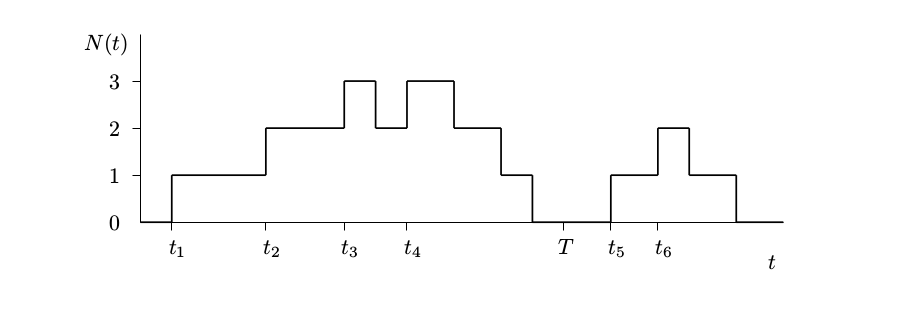
\includegraphics[width=\textwidth]{./imgs/fig2.png}
			\caption{Trayectoria de $N_t$}
			\label{fig:enet}
		\end{center}
	\end{figure}
	
	Mientras que los tiempos de espera son períodos de tiempo, también se pueden observar como rectángulos 
	de altura 1 en la gráfica de ${\Delta(t)}$. Así, la longitud $W_n$ es también área $W_n$. Para cada $t$, 
	$N_t$ es simplemente el número de rectángulos de tiempo de espera que contienen el punto $t$.
	
	Tenemos por tanto un modelo de colas, con $t_n, W_n $ y $ N_t$ variables aleatorias; lo que nos lleva
	trivialmente a asumir que  $\{t_n\}_{n\ge 1}, \{W_n\}_{n\ge 1}, \{N_t\}_{t\ge 0}$ son procesos estocásticos.
	
	Por lo general, en nuestro caso se suelen hacer las siguientes suposiciones :
	\begin{itemize}
		\item $W_n$ tiene la misma distribución para todo $n$.
		\item $N_t$ tiene la misma distribución para todo $t$.
	\end{itemize} 
	
	Llegados a este punto hemos de remarcar que existen realmente dos versiones de la Ley de Little: 
	
	\begin{itemize}
		\item La versión que relaciona el tiempo de espera medio y la cantidad media de clientes en la cola: 
		la más conocida y a que trataremos en el trabajo.
		\item La versión estacionaria que relaciona los valores esperados de $W_W$ y $N$ través de la esperanza. 
	\end{itemize}
	
	Damos a continuación una idea intuitiva del primer teorema, que puede contribuir a su comprensión.
	
	\begin{rmk*}
		De ahora en adelante omitiremos el punto del espacio muestral en el que estamos. Esto no afecta 
		en absoluto a nuestro trabajo y simplifica la notación al no tener que acarrerar la dependencia 
		explícita del mismo: Por ejemplo, escribimos $W_n$ en lugar de $W_n(\omega)$. 
	\end{rmk*}
	
	El área rectangular $W_n$ es la contribución al área bajo $N_t$ que es realizada por el cliente $n$-ésimo. 
	Ahora considerese el área bajo $N_t$ en algún intervalo $]0,T[$, donde como en las figuras \ref{fig:deltat}
	y \ref{fig:enet}, $T$ tiene la propiedad de que $N_T = 0$. Para cualquier $T$ de esa forma, este área puede 
	escribirse como una integral o una suma:
	
	\[\int_{0}^{T} N_t dt=\int_{0}^{T} \sum_{i=1}^{\Delta (t)} I_i(t) dt \underset{permutando}{=}\sum_{i=1}^{\Delta (t)} W_i\]
	
	Se puede observar en la figura \ref{fig:deltat} en $\Delta(T) = 4$.
	
	Para cualquier $T$ donde $N_T > 0$, la anterior igualdad no es cierta porque una porción de al menos un 
	rectángulo en la suma contribuye al área bajo $N_t$ después de $T$. 
	%En este caso, la suma - integral $\equiv$ error $\geq 0$.
	
	Entonces definimos la media de estas cantidades a largo plazo como límites, cuando existan, denominándolos
	como siguen:
	
	\begin{itemize}
		\item $L = \lim_{T\to \infty}\frac{1}{T} \int_{0}^{T} N_t dt$
		\item $W_W = \lim_{n\to \infty}\frac{1}{n} \sum_{i=1}^{n} W_i$
		\item $\lambda = \lim_{t\to \infty}\frac{\Delta(t)}{t}$
	\end{itemize}
	
	Donde conceptualmente estamos haciendo referencia a:
	\begin{itemize}
		\item $L$ es el número medio de clientes en el sistema,
		\item $W_W$ es el tiempo medio de espera (de los clientes en el sistema), y
		\item $\lambda$ es la tasa de llegada 
	\end{itemize}
	Es de destacar que  $L$ y $W_W$ son las dos medidas de rendimiento más comunes para una cola.
	
	
	Tenemos ya todos los elementos para formular el teorema de Little:
	\begin{theorem*}{\textbf{Teorema de Little}}\\
		Si los límites $\lambda$ y $W_W$ existen y son finitos, entonces $L$ existe y es finito, donde 
		\[L = \lambda W_W\]
	\end{theorem*}
	
	La idea intuitiva de este resultado es la relación que apúntabamos antes: para cualquier $T$ (donde ahora $N_T \geq 0$) escribimos:
	\[ \frac{\int_{0}^{T} N_t dt}{T}=\frac{\sum_{i=1}^{\Delta (t)} W_i(t)}{T}-\frac{error}{T}=\frac{\Delta(t)}{T}\frac{\sum_{i=1}^{\Delta (T)} W_i(t)}{\Delta(T)}-\frac{error}{T}   \]
	A medida que T se hace grande, la primera cantidad entre paréntesis a la derecha se aproxima a $\lambda$, la segunda a $\omega$, 
	y el producto se acerca $\lambda\omega$. Por lo tanto, el teorema se obtendría si el término a la derecha 
	se aproxima a 0 cuando $T\rightarrow\infty$. El término de error no tendría porqué hacerse pequeño, 
	sólo crecer más lentamente que T.
	Teniendo esta idea en mente, podemos proceder a demostrar el resultado formalmente:
	
	\begin{proof}
		Motivados por las figuras \ref{fig:deltat} y \ref{fig:enet}, encontramos obvias las siguientes desigualdades:
		\begin{equation}
		\sum_{\{i:t_i+W_i\leq T\}}^{} W_i\leq\int_{0}^{T}N_t dt\leq \sum_{i=1}^{\Delta(T)} W_i
		\label{DesiLi}
		\end{equation}
		donde la suma a la izquierda está por debajo de aquellos rectángulos de espera que han terminado en $T$.
		Ahora dividimos la expresión por $T$ y hacemos tender $T\rightarrow\infty$. La expresión de la derecha 
		tiene límite $\lambda W_W$, lo que implica que la integral tiene $\lim_{sup} \leq \lambda W_W$. Si conseguimos 
		demostrarlo para el inferior concluiremos la demostración. Con ese fin, necesitamos dos resultados 
		preliminares. Primero, escribimos: 
		
		\[ \frac{W_n}{n}=\frac{1}{n}\sum_{i=1}^{n}W_i-\left(\frac{n-1}{n}\right) \left(\frac{1}{n-1}\right)\sum_{i=1}^{n-1}W_i \] 
		
		Para $W_W$ finito, esta expresión tiene límite $0$ si $n \rightarrow \infty$. Es decir,
		
		\[ \lim_{n\to\infty} W_n / n = 0. \]
		
		Si, ahora, $\lambda$ es finito, esto implica $t_n \rightarrow \infty$ y, $\Delta(t_n)/t_n \rightarrow  \lambda$ como $n \rightarrow \infty$. Si los tiempos 
		de llegada son distintos escribiríamos, $\Delta(t_n)=n$; de lo contrario, $\Delta(t_n)\geq n$, y escribimos:
		
		\[ \frac{W_n }{t_n} = \frac{W_n }{n}\frac{n }{t_n}\leq \frac{W_n }{n}\frac{\Delta(tn)}{t_n} \]
		tenemos por tanto:
		\[ \lim_{n\to\infty} W_n / t_n = 0. \]
		
		Para cualquier $\epsilon> 0$, el anterior limite implica que para algún $m$ finito y todo $i > m$, $W_i < t_i \epsilon$ 
		y $t_i + W_i <t_i (1 + \epsilon)$. Así, $t_i \leq T / (1 + \epsilon) \Longrightarrow t_i + W_i \leq T$ para 
		cada $i> m$,lo que nos da esta cota inferior en la expresión de la izquierda en \ref{DesiLi}:
		
		\begin{equation}
		\sum_{i=1}^{\Delta\left(\frac{T}{1+\epsilon}\right)} W_i-\sum_{i=1}^{m} W_i\leq \sum_{\{i:t_i+W_i\leq T\}}^{} W_i
		\label{eq:desiLi2}
		\end{equation}
		
		Ahora dividimos por $T$ y hacemos $T\rightarrow +\infty$, notando que el segundo término de la izquierda es una
		constante. El lado izquierdo de \ref{eq:desiLi2} tiene límite $ \lambda W_W / (1 + \epsilon)$, lo que implica 
		el lado derecho tiene $\lim_{inf} \ge \lambda W_W / (1 + \epsilon))$. Debido a que $\epsilon$ puede ser arbitrariamente 
		pequeño, y combinando limite superior e inferior, concluimos la prueba.
	\end{proof}
	\subsection{Ejemplo de aplicación}
	Supongamos que tenemos dos sistemas de colas distintas, de hecho podemos suponer que tienen diferencias considerables: podemos usar un sistema multicola con dos servidores y un sistema con una sola cola. Entonces como afectaría este cambio a los clientes? En particular, ¿tendremos algún efecto en el tiempo de espera medio?
	
	Si suponemos que los tiempos de llegada y de servicio están fijos, lo que realmente estamos haciendo es cambiar el orden de servicio: con un modelo de una sola cola los clientes estarían servidos según la disciplina FIFO. Con el modelo de varias colas serían una reordenación del primer caso.
	
	Si suponemos que los tiempos de servicio están idénticamente distribuidos entonces, los tiempos de servicio servidos en el orden determinado también lo serán. Así la distribución del número de clientes en el sistema no cambiará. Más específicamente tendremos que la media del numero de personas y la tasa de llegada serán las mismas por lo que la Ley de Little nos dice que el tiempo medio de espera será el mismo, con lo que aunque la distribución que sigue el tiempo de espera puede variar, los clientes en general, no notarán diferencia.
	
	\section{Modelos particulares}
	\subsection{D/D/1}
	Tenemos un tiempo entre llegadas constante $\tau = \frac{1}{\lambda}$ y un tiempo de servicio constante $S = \frac{1}{\mu}$.
	
	En este caso, la intensidad de tráfico será $a=\frac{\lambda}{\mu}$, y por ser $c = 1$, el aprovechamiento del servidor es el mismo, $\rho = a$.
	
	\subsubsection{Caso $\lambda > \mu$}
	Intuitivamente, la cola será inestable y no podrá servir todas las peticiones. 
	
	Se tiene $a > 1$, $\rho > 1$.
	
	\begin{fact*}
		Notando $Q_n$ al tiempo de espera del $n$ ésimo cliente, tenemos que \[Q_1 = 0, \qquad Q_n = \left(\frac{1}{\mu} - \frac{1}{\lambda}\right)n, \quad \forall n\ge 2\]
	\end{fact*}
	
	\begin{proof}
		Veámoslo por inducción:
		
		El segundo cliente, que llega en tiempo $\frac{2}{\lambda}$ al sistema, debe esperar que el cliente que entró en tiempo $\frac{1}{\lambda}$ sea servido,
		esto es $\frac{1}{\mu} - \frac{1}{\lambda}$
		
		Supuesto que $Q_{n-1}$ cumple esa relación, el $n$ ésimo cliente entra $\frac{1}{\lambda}$ unidades de tiempo
		más tarde que el $n-1$ ésimo y deberá esperar a que el $n-1$ ésimo sea servido para poder él ser servido, esto es,
		deberá esperar $Q_{n-1} + \frac{1}{\mu} - \frac{1}{\lambda} = \left(\frac{1}{\mu} - \frac{1}{\lambda}\right)n$
	\end{proof}
	
	\begin{corollary*}
		El tiempo de espera total para el $n$ ésimo cliente es:
		
		\[W_1 = \frac{1}{\mu}, \qquad W_n = \left(\frac{1}{\mu} - \frac{1}{\lambda}\right)^n + \frac{1}{\mu} \quad n\in \mathbb{N}\]
	\end{corollary*}
	
	\begin{fact*}
		En un instante $t$ el número de clientes en el sistema será: 
		\[N_t = \left\{\begin{array}{lcc}
		0, && t < \frac{1}{\lambda}\\
		\lfloor t\lambda \rfloor - \left\lfloor\left(t-\frac{1}{\lambda}\right)\mu\right\rfloor, && \text{otro caso}
		\end{array}\right.\]
	\end{fact*}
	
	\begin{proof}
		Trivial.
	\end{proof}
	
	
	\subsubsection{Caso $\lambda \le \mu$}
	
	Se tiene $a < 1$, $\rho < 1$.
	
	\begin{fact*}
		Se tiene $\forall n\in \mathbb{N}$:
		
		\begin{align*}
		Q_n = 0\\
		W_n = \frac{1}{\mu}
		\end{align*}
	\end{fact*}
	
	\begin{corollary*}
		El tiempo de espera total para el $n$ ésimo cliente es únicamente el tiempo en ser servido:
		
		
	\end{corollary*}
	
	\begin{fact*}
		En un instante $t$ el número de clientes en el sistema será: 
		\[N_t = \left\{\begin{array}{lcc}
		0, && t < \frac{1}{\lambda}\\
		0, && t \ge \frac{1}{\lambda}, t \in \left]\frac{n-1}{\lambda} + \frac{1}{\mu}, \frac{n-1}{\lambda} + \frac{1}{\lambda}\right[\\
		1, && \text{otro caso}
		\end{array}\right.\]
	\end{fact*}
	
	En el caso particular $\lambda = \mu$, se tiene $N_t = 1$ constantemente para $t\ge \frac{1}{\lambda}$
	
	\subsection{M/M/1}
	
	En este modelo consideramos un patrón de llegadas aleatorio y tiempo de servicio siguiendo una distribución 
	exponencial. El tiempo de llegada no depende de los clientes en el sistema, por proposición \ref{fact:exp-markov}
	y, si tenemos en cuenta el teorema \ref{th:poisson-probs}, la probabilidad de que se produzca una llegada 
	en un intervalo de tiempo $h>0$ viene dada por:
	
	\begin{align*}
	& e^{-\lambda h}(\lambda h)= \left(1-\lambda h+\frac{(\lambda h)^2}{2!}- \dots\right) \lambda h = \\
	& =\lambda h-(\lambda h)^2+\frac{(\lambda h)^3}{2!}-\dots+(-1)^n\frac{(\lambda h)^n}{(n-1)!} + \ldots = \lambda h+o(h)
	\end{align*}
	
	Por tanto tenemos :
	\begin{equation*}
	\lambda_n=\lambda, \quad n=0,1,2,\dots
	\end{equation*}
	
	Por hipótesis la distribucion que sigue el tiempo de servicio viene dada por:
	\begin{equation*}
	W_S[t] = P[S\leq t] = 1-e^{-\mu t}, \quad t\ge 0.
	\end{equation*}
	
	Por tanto si un cliente está recibiendo el servicio, la probabilidad de que el servicio sea completado en un corto periodo de tiempo, $h$, viene dada por:
	\begin{equation*}
	1-e^{-\mu h} = 1 - \left(1-\mu h+\frac{(\mu h)^2}{2!}- \dots\right)=\mu h +o(h)
	\end{equation*}
	
	Donde hemos usado la propiedad de falta de memoria de la distribucion exponencial, omitiendo los servicios ya acabados)\\
	Por tanto:
	\begin{equation*}
	\mu_n=\mu, \quad n=0,1,2,\dots
	\end{equation*}
	
	Así, podemos deducir el diagrama de estado-transición para el sistema de colas M/M/1. Además dado que $\lambda/\mu=\rho$ utilizando la serie calculada en \ref{eq:stabseries} nos queda que:
	\begin{equation*}
	Z=1+\rho+\rho^2+\dots+\rho^n+\dots=\frac{1}{(1-\rho)}
	\end{equation*}
	
	Hemos asumido que $\rho<1$ por lo que una solución estacionaria existe.
	Para sumar la serie de S hemos usado la suma de la serie geométrica ampliamente conocida.
	Así por la definicion de \ref{eq:relp0} y \ref{p_n=p_0*}
	\begin{equation}
	p_n=P[N=n]=(1-\rho)\rho^n, n=0,1,2...
	\label{eq:p_n}
	\end{equation}
	
	Podemos observar que \ref{eq:p_n} es la funcion masa de probabilidad de una variable aleatoria geométrica;esto
	es, $N$ sigue una distribucion geométrica con $p=1-\rho$ y $q=p$. Por tanto podemos usar para obtener $L$ 
	y $\sigma_n^2$:
	\begin{equation*}
	L=E[N]=q/p=\frac{\rho}{(1-\rho)}
	\end{equation*}
	
	\begin{equation*}
	\sigma_n^2=\frac{\rho}{(1-\rho)^2}
	\end{equation*}
	
	Usando la Ley de Little \ref{little}:
	\begin{equation*}
	W=E[\omega]=\frac{L}{\lambda}=\frac{W_s}{(1-\rho)}
	\end{equation*}
	
	Equvalentemente como \[ W_q=E[q]=W-W_s=\frac{\rho W_s}{(1-\rho)} \] podemos volver a usar la Ley de Little 
	para obtener:
	\begin{equation*}
	L_q=E[N_q]=\lambda W_q=\frac{\rho^2}{(1-\rho)}.
	\end{equation*}
	
	Podemos tambien calular utilizando \ref{p_n} la probabilidad de que el servidor esté ocupado:
	\begin{equation*}
	P[\textbf{Servidor ocupado }]=1-P[N=0]=1-(1-\rho)=\rho
	\end{equation*}
	Por la ley de grandes números esta probabilidad puede ser interpretada como la fracción de tiempo que el 
	servidor está ocupado; de hecho podríamos considerar llamar a $\rho$ "Utilización del servidor".
	
	Tenemos ya los cuatro parámetros más utilizados para medir la rendimiento de un sistema de colas 
	$W, W_q, L y L_q$, así como el la funcion masa de probabilidad, $p_n$, de una cantidad en el sistema, $N$. 
	
	Para el sistema $M / M / 1$, también podemos obtener la distribución exacta de $\omega$ y q.
	
	Si un cliente que llega no encuentra clientes en el sistema, $(N = 0)$, entonces no hay cola para el 
	servicio, por lo que $W_q [O] = P [q = 0] = P [N = 0] = 1 - \rho$.
	
	Así, $W_q [.]$ Tiene una concentración o masa de probabilidad en t = O. 
	Sin embargo,si un cliente llega cuando n clientes ya están en el sistema, entonces tiene que esperar a
	través de n tiempos de servicio (que recordemos siguen una distribución exponenciales); eso es el tiempo
	de espera condicional en la cola, dada una llegada a la misma con n clientes ya en el sistema, vendrá dado por
	\[q = s_1 + s_2 + \dots + s_n\]
	
	Donde $s_n$ son n exponenciales independientes distribuidas de forma idéntica cada una con media $1 / \lambda$.  Por tanto usando las propiedades de la distribución gamma, $q$ tiene una distribución gamma con los parámetros n y $\lambda$, que significa que la función de densidad de probabilidad ,condicionada al caso propuesto, de $q$, está dada por
	\begin{equation*}
	f_{q,n}(t)=\mu e^{-\mu t} \frac{(\mu t)^{n-1}}{(n-1)!}
	\end{equation*}
	
	Así, si n> 0,podemos calcular la probabilidad como:
	\begin{equation*}
	P[q\leq t|N=n]=\int_{0}^{t}\frac{\mu^nx^{n-1}e^{-\mu x}}{(n-1)!}dx
	\end{equation*}
	
	Siguiendo la ley de probabilidad total:
	\begin{equation*}
	P[0<q\leq t]=\sum_{n=1}^{\infty}P[q\leq t|N=n]P[N=n]
	\end{equation*}
	
	Operando podemos obtener, finalmente:
	\begin{equation*}
	P[0<q\leq t]=\rho[1-e^{-t/W}]
	\label{finaleqP}
	\end{equation*}
	
	
	Ya hemos demostrado que $W_q [O] = 1 - p$. Si t> 0, podemos usar \ref{finaleqP} para calcular 
	\[W_q [t]=P [q = 0] + P [O <q \leq t]= 1 - \rho + \rho [1 - e^{- t / W}]=1\rho[1-e^{-t/W}\]
	
	El tiempo medio de espera en cola es de particular interés por los sistemas de colas en los que las personas son los clientes.Es de sentido común pensar que, si las personas se mantienen esperando demasiado tiempo en la cola para un servicio, éstas puedan cansarse y abandonar la cola; es decir, abandonar la cola sin haber recibido el servicio. La gente no esperará indefinidamente por ningún tipo de servicio.
	
	De hecho podemos calcular como funciona nuestro caso ante esta idiosincrasia. Usando las propiedades de condicionamiento:
	\begin{equation*}
	W_q = P [q = 0] E [q|q = 0] + P [q> 0]E [q|q> 0] = (1 - \rho)  0 + \rho E [q|q> 0].
	\end{equation*}
	
	Lo que nos lleva a:
	\begin{equation*}
	\frac{W_q}{\rho}=\frac{W_s}{1-\rho}=W= E [q|q> 0].
	\end{equation*}
	Este resultado, dado que $W=W_q+W_s$, se puede interpretar de la siguiente manera: De media un cliente esperando al servicio permanecerá en la cola el tiempo medio de servicio más que lo que espera un cliente medio.
	Es más, la función de distribución de $W[.]$ se puede obtener de igual forma que hicimos con $W_q[.]$. Con lo que podemos concluir que $\omega$ sigue una distribución exponencial lo que nos permite calcular los percentiles de la misma.
	
	\section{Ejemplos y simulaciones}
	\subsection{La paradoja del tiempo de espera}
	Vemos ahora un ejemplo de un resultado que contradice al sentido común. Supongamos que estamos en la parada del autobús, y sabemos que el autobús pasa por la parada con una frecuencia media de $\lambda$, esto es, de media pasa cada $\alpha=\frac{1}{\lambda}$ minutos. ¿Cuál es la esperanza del tiempo que pasará hasta que llegue el siguiente autobús?
	
	La intuición dice que de media el autobús llegará en la mitad del intervalo de tiempo entre autobuses, $\frac{\alpha}{2}$. Sin embargo, se puede comprobar que esto es cierto sólo en el caso de que los autobuses pasen cada 15 minutos exactamente, esto es, cuando el tiempo entre llegadas es determinístico. A continuación vemos la respuesta real al problema.
	
	\begin{fact*}
		Si los tiempos entre llegadas de autobuses son independientes e idénticamente distribuidos, $\tau_n = \tau \quad \forall n \in \mathbb{N}$, entonces la esperanza del tiempo que tarda en llegar el autobús es
		$$\frac{\alpha}{2} + \frac{\sigma^2}{2\alpha} $$
		donde $\alpha$ es la media de $\tau$ y $\sigma^2$ es la varianza de $\tau$.
	\end{fact*}
	
	\begin{proof}
		% Repasar cuentas
		Sea $F$ la función de distribución de $\tau$, y sean $t_1 < \cdots < t_n < \cdots$ los tiempos de llegada del autobús. Llamamos $W_t(x)$ a la probabilidad de que el tiempo que tarde en llegar un autobús sea menor o igual que $x$.
		
		Esto sucederá cuando llegue al menos un autobús en el intervalo $\rbrack t, t+x\rbrack$. Lo dividimos en sucesos disjuntos considerando la posibilidad de que el $n$-ésimo autobús sea el último autobús que llega durante dicho intervalo, esto es, si $t_n \in \rbrack t, t+x \rbrack$ y $t_{n+1} \notin \rbrack t, t+x \rbrack$. La expresión anterior equivale a que $t < t_n \leq t+x < t_{n+1}$, luego sumando para cada $n \in \mathbb{N}$, se tiene que
		\begin{align*}
		W_t(x) &= \sum_{n=1}^\infty P[t < t_n \leq t+x < t_{n+1}] \\
		&= \sum_{n=1}^\infty \int_t^{t+x} [1-F(t+x-u)]dP[t_n \leq u] \\
		&= \int_t^{t+x} \sum_{n=1}^\infty [1-F(t+x-u)]dP[t_n \leq u]
		\end{align*}
		Se puede comprobar que
		$$ \sum_{n=1}^\infty P[t_n \leq t] = \lambda = \frac{t}{\alpha} $$
		ya que es equivalente al número de autobuses que se espera que lleguen durante el intervalo $\rbrack 0,t \rbrack$.
		Por tanto, en la fórmula anterior se tiene
		\begin{align*}
		W_t(x) &= \int_t^{t+x} [1-F(t+x-u)]\frac{u}{\alpha}du \\
		&= \frac{1}{\alpha}\int_0^x [1-F(y)]dy
		\end{align*}
		
		Por tanto, podemos calcular el tiempo esperado que tardará en llegar el autobús:
		$$ \int_0^\infty xdW_t(x) = \frac{1}{\alpha}\int_0^\infty x[1-F(x)]dx = \frac{\alpha^2+\sigma^2}{2\alpha}$$
	\end{proof}
	
	Con el resultado de esta proposición se demuestra que el tiempo esperado que tardará en llegar el autobús depende no sólo de la media sino también de la varianza. Por tanto, si consideramos distribuciones habituales de $\tau$, se tiene:
	\begin{itemize}
		\item Si $\tau=\lambda$ constante, entonces, el tiempo esperado es $\frac{\lambda}{2} + \frac{0}{2\lambda} = \frac{\lambda}{2}$.
		\item Si $\tau \sim exp(\lambda)$, entonces, el tiempo esperado es $\frac{\lambda}{2} + \frac{\lambda^2}{2\lambda} = \lambda$.
		%%\item Si $\tau \sim E(k,\lambda)$, entonces, el tiempo esperado es $\frac{k}{2\lambda} + \frac{k\lambda}{2\lambda^2k} = \frac{k}{2\lambda} + \frac{1}{2\lambda} = \frac{k+1}{2\lambda}$.
	\end{itemize}
	
	
	\newpage
	\begin{thebibliography}{10}
		\expandafter\ifx\csname url\endcsname\relax
		\def\url#1{\texttt{#1}}\fi
		\expandafter\ifx\csname urlprefix\endcsname\relax\def\urlprefix{URL }\fi
		\expandafter\ifx\csname href\endcsname\relax
		\def\href#1#2{#2} \def\path#1{#1}\fi
		
		\bibitem{Allen}
		Arnold O.Allen (1990)\\
		Probability, Statistics and Queueing Theory with Computer Science Applications\\
		Academic Press
		
		\bibitem{Gross}
		Donald Gross, John F.Shortle, James M.Thompson, Carl M.Harris (2008)\\
		Fundamentals of Queueing Theory\\
		Wiley
		
		\bibitem{Gunavathi}
		P.Kandasamy, K.Thilagavathi, K.Gunavathi\\
		Probability and Queueing Theory (2010)\\
		S. Chand \& Company
		
		\bibitem{Wolff}
		Ronald W. Wolff\\
		Little's law and Related Results (2011)\\
		University of California at Berkeley
	\end{thebibliography}
	
\end{document}
